\begin{ledgroupsized}[r]{120mm}
\footnotesize
\pstart
\noindent\textbf{Überlieferung:}
\pend
\end{ledgroupsized}
\begin{ledgroupsized}[r]{114mm}
\footnotesize
\pstart \parindent -6mm
\makebox[6mm][l]{\textit{L}}%
Konzept:
LH~XXXVII~5 Bl.~195. 
Ein Blatt~4\textsuperscript{o};
Papiererhaltungsmaßnahmen;
alle Ränder bis auf den rechten beschnitten.
Zwei Seiten; Textfolge: Bl.~195~r\textsuperscript{o}, Bl.~195~v\textsuperscript{o}, Schlussteil auf Bl.~195~r\textsuperscript{o} (am Rand, senkrecht zur Schreibrichtung). 
\pend
\end{ledgroupsized}
\vspace{5mm}
\begin{ledgroup}
\footnotesize
\pstart
\noindent%
\textbf{Datierungsgründe:}
Wegen der Erwähnung eines Schreibens an 
\indexN{\textls{Papin} (Papinus), Denis 1647\textendash1713}Denis Papin 
im Schlusssatz von N.\;\ref{60358}
("Nota de hoc loquor et in Ep. ad Papinum data ante med. octob. 1698")
kann von einer Entstehung des Konzeptes kurz nach dem Brief ausgegangen werden,
zumal die Bezugnahme im Präsens erfolgt ("loquor").
Es handelt sich um den Brief \cite{01501}\textit{LSB} III~7, N.\;237, 
der die Thematik von N.\;\ref{60358} (das Kraftmaß und die Rolle der Elastizität beim Stoß)
bes. auf S.\;924.20\textendash925.3 aufgreift.
\pend
\end{ledgroup}
\selectlanguage{latin}
\vspace{8mm}
\pstart%
\noindent%
\edlabel{37_05_195_1a}%
\edtext{}{%
{\xxref%
{37_05_195_1a}{37_05_195_1b}}%
\lemma{}\Afootnote{\textit{Am oberen Rand}: %
Hic explicantur celeritates\indexS{celeritas residua} quae in corporibus duobus concurrentibus manent residuae, dum se urgent et ictu comprimunt.}}%
\edtext{\href{\Scan{LH_37_05_195r}}%
{\lbrack195~r\textsuperscript{o}\rbrack}%
\edlabel{37_05_195_1b} Mutatio}{%
\lemma{\href{\Scan{LH_37_05_195r}}%
{\lbrack195~r\textsuperscript{o}\rbrack}}\Bfootnote{%
\textit{(1)}~Cum corpus a corpore impellitur, mutatio fit instan %
\textit{(2)}~Mutatio~\textit{L}}}
notabilis instantanea\indexS{mutatio instantanea} esse non potest. Itaque non dantur Atomi,\indexS{atomus} et 
cum corpus incurrit corpori non ante devenit ad quietem,\indexS{quies} quam decreverit per omnes celeritates 
medias inter suam et quietem, nec rursus transit ad motum contrarium,\indexS{motus contrarius} quam 
\edtext{ubi rursus a quiete}{\lemma{ubi}\Bfootnote{%
\textit{(1)}~ad quiete %
\textit{(2)}~rursus a quiete~\textit{L}}}
per omnes celeritates medias ad eum 
\edlabel{37_05_195_2a}%
\edtext{}{%
{\xxref%
{37_05_195_2a}{37_05_195_2b}}%
\lemma{exurrexerit.}\Bfootnote{%
\textit{(1)}~Hinc corpus concurrens cum altero comprimitur %
\textit{(2)}~Hinc %
\textit{(3)}~Hinc~\textit{L}}}%
exurrexerit.
\pend
\begin{edfigure}%
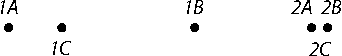
\includegraphics[scale=1]{gesamttex/edit_VIII-4/images/LH_37_05_195_d1_195r.pdf}
\edcaption[0pt]{\lbrack\textit{Fig.~1}\rbrack}
\end{edfigure}
\pstart
Hinc%
\edlabel{37_05_195_2b}
si duo corpora, quae supponantur elastica,\indexS{corpus elasticum} ex hoc
\edtext{principio, accedentibus}{\lemma{principio,}\Bfootnote{%
\textit{(1)}~accedente regula deter %
\textit{(2)}~accedentibus~\textit{L}}}
\edtext{dynamicis\indexS{dynamica} nostris,}{%
\lemma{dynamicis nostris}%
\Cfootnote{Gemeint sind möglicherweise die Entwürfe \cite{01354}\textit{Dynamica de potentia} von 1689 oder das \cite{02032}\textit{Specimen Dynamicum} von 1695.}}
definiri potest, quantum utrique supersit motus. Sint 
\edtext{corpora \textit{a}}{%
\lemma{corpora}%
\Bfootnote{%
\textit{(1)}~\textit{A} et \textit{B}. Tens %
\textit{(2)}~\textit{a}~\textit{L}}}
et \textit{b}, celeritates ante ictum \textit{v} et \textit{e}, quas pono tendere ad easdem partes, nam si secus sit,
\edtext{pro affirmativa celeritatis}{\lemma{pro}\Bfootnote{%
\textit{(1)}~affirmativis celeritatis quantitatibus alterius %
\textit{(2)}~affirmativa celeritatis~\textit{L}}}
alterius quantitate
substituetur 
\edtext{negativa. Celeritas respectiva,\indexS{celeritas respectiva} seu}{\lemma{negativa.}\Bfootnote{%
\textit{(1)}~Centri gravitatis celeritas erit $v+e,:2$  %
\textit{(2)}~Celeritas respectiva %
\textit{(a)}~est %
\textit{(b)}~, seu~\textit{L}}}
qua mutatur distantia, 
\edtext{est $v-e$.}{\lemma{est}\Bfootnote{%
\textit{(1)}~$v+e$. %
\textit{(2)}~$v-e$.~\textit{L}}}
Ea distribuenda est inter corpora, ut sit celeritas ipsius \textit{a} ad celeritatem ipsius \textit{b}, ut \textit{b} 
ad \textit{a}; seu 
\edtext{ut $1:a$}{\lemma{ut}\Bfootnote{%
\textit{(1)}~$\displaystyle\displaystyle\frac{1}{a}$ %
\textit{(2)}~$1:a$~\textit{L}}}
ad $1:b$, eritque celeritas
\edtext{ipsius \textit{a}, $\displaystyle\displaystyle\frac{b}{a+b}v-e,$}{\lemma{ipsius \textit{a},}\Bfootnote{%
\textit{(1)}~\rule[-2.1ex]{0pt}{5.4ex}%
$\displaystyle\frac{b}{a+b}v+e,\displaystyle\frac{a+b}{a}$ %
\textit{(2)}~$\displaystyle\frac{b}{a+b}v-e,$~\textit{L}}}
et ipsius \textit{b}  
\edtext{celeritas erit $\displaystyle\displaystyle\frac{a}{a+b}v-e.$}{\lemma{celeritas erit}\Bfootnote{%
\textit{(1)}~$\displaystyle\frac{a}{a+b}v+e,(a^2+b).$ %
\textit{(2)}~$\displaystyle\frac{a}{a+b}v-e.$~\textit{L}}}
Et vis
\edtext{ictus\indexS{vis ictus} erit $\displaystyle(v-e:,a+b)\,\protect\fbox{2}$, in $aab+bba$\lbrack,\rbrack}{\lemma{ictus erit}\Bfootnote{
\textit{(1)}~$\overline{v+e}^2:a,+$ %
\textit{(2)}~$(\displaystyle\frac{1}{a}+\displaystyle\frac{1}{b})(\overline{v+e}^2)(a+b)^2$  
\textit{(3)}~$\displaystyle\frac{a^2}{\overline{a+b}^2}\overline{v+e}^2+\displaystyle\frac{b^2}{\phantom{a+b}}$  
\textit{(4)}~\rule[-2.8ex]{0pt}{6.9ex}%
$\displaystyle\frac{ab^2}{\overline{a+b}^2}$
\textit{(5)}~$(abb)((v+e:a+b))$
\textit{(6)}~(\protect\vphantom)\textit{v}
\textit{(a)}~$+e$
\textit{(b)}~$-e:,a+b\protect\vphantom()\protect\fbox{2}$, in $aab+bba$~\textit{L}}}
qua scilicet tensio\indexS{tensio elastri} elastri\indexS{elastrum} integra
\edtext{constat. Seu}{\lemma{constat.}\Bfootnote{\textit{(1)}~Se %
\textit{(a)}~si
\textit{(aa)}~vi %
\textit{(bb)}~tensio
\textit{(b)}~si 
\textit{(2)}~Sed cum tensio non statim sit perfecta, ideo parte tantum peracta ut in navi, habebimus
\textit{(3)}~Vis aute %
\textit{(a)}~centri gravitatis eri %
\textit{(b)}~tota erat $av^2+be^2$ a qua si detrahas vim ictus $\overline{v+e}^2$, 
\textit{(aa)}~$a+2b+b+2a$ %
\textit{(bb)}~$a+2b+(b^2:a)+(a^2:b)+2a+b$
\textit{(aaa)}~seu $\overline{v+e}^2$, $3a+3b+b^2:a+a^2:b$ seu
\textit{(bbb)}~seu explicatius erit %
\textit{(4)}~Seu~\textit{L}}}
dividendo numeratorem et nominatorem per $a+b$
\edtext{fit $\overline{v-e}^{2},ab:,a+b$,}{\lemma{fit}\Bfootnote{%
\textit{(1)}~$\overline{v+e}^2,ab:,a+b$ %
\textit{(2)}~$\overline{v-e}^2,ab:,a+b$~\textit{L}}}
vis 
ictus\indexS{vis ictus} seu tensionis\indexS{vis tensionis totalis} totalis seu 
\edtext{explicatius: $abvv-2abve+abee,:,a+b$. Hanc vim auferendo a vi tota\indexS{vis tota}}{\lemma{explicatius:}\Bfootnote{%
\textit{(1)}~$abvv+$ %
\textit{(2)}~$abvv-2abve+abee,:,a+b$ 
\textit{(a)}~Haec vis auferenda a vi tota, %
\textit{(aa)}~fiet %
\textit{(bb)}~restabit vis directionis %
\textit{(b)}~Hanc vim auferendo a vi tota~\textit{L}}}
$avv+bee$, seu ab $aavv+abvv+abee+bbee,:,a+b$, restabit $aavv+2abve+bbee,:,a+b$ seu $\overline{av+be}^{2}\!:,a+b$, quae est vis directionis;\indexS{vis directionis} 
\edtext{quam summa}{\lemma{quam}\Bfootnote{%
\textit{(1)}~dividendo per sum %
\textit{(2)}~summa~\textit{L}}}
corporum habet mota celeritate
centri gravitatis\indexS{celeritas centri gravitatis}. 
Dividendo ergo hanc vim per summam 
\edtext{corporum, et}{\lemma{corporum,}\Bfootnote{%
\textit{(1)}~prodit $\overline{(av-be):(a+b)}^2$ cujus latus est $av-be$ %
\textit{(2)}~et~\textit{L}}}
quotientis sumendo radicem prodit celeritas centri gravitatis\indexS{celeritas centri gravitatis} $av+be,:,a+b$; quae debet esse \textit{\ind{1}C\ind{2}C}. 
Nempe $\ind{1}C\ind{2}C=\ind{1}C\ind{1}B+\ind{1}B\ind{2}B$ 
jam \textit{\ind{1}B\ind{2}B} est \textit{e} et \textit{\ind{1}C\ind{1}B} est ad \textit{\ind{1}A\ind{1}B} id est ad $v-e,$ ut \textit{a} ad $a+b$.
Ergo \textit{\ind{1}C\ind{1}B} est $a,v-e,:,a+b$ et \textit{\ind{1}C\ind{2}C} est $\displaystyle av\ \ovalbox{-ae+ae}+be,:,a+b$. 
Ergo est consensus.
\pend
\pstart
Sed si tensio\indexS{tensio} nondum absoluta sit, 
\edtext{videamus quae pro facto gradu tensionis\indexS{tensio} residua}{%
\lemma{videamus}%
\Bfootnote{%
\textit{(1)}~quis pro facto gradu tensionis residuus %
\textit{(2)}~quae \lbrack...\rbrack\ residua~\textit{L}}}
sit celeritas et directio in quovis corporum, interea dum se urgent. 
Sit ergo tensionis vis;\indexS{vis tensionis} qualis fuisset  
\edtext{si velocitas}{\lemma{si}\Bfootnote{%
\textit{(1)}~corpora eandem %
\textit{(2)}~vis %
\textit{(3)}~velocitas~\textit{L}}}
respectiva\indexS{velocitas respectiva} fuisset minor quam $v-e$, seu quam \textit{\ind{1}A\ind{1}B}. 
Ponamus fuisse $v-e-f$. Posito $e+f$ non excedere
\edtext{\textit{v}, et}{\lemma{\textit{v},}\Bfootnote{%
\textit{(1)}~et utcunque %
\textit{(2)}~et~\textit{L}}}
in calculo priore pro \textit{e} substituendo $e+f$, fiet vis tensionis
\edtext{factae,\indexS{vis tensionis factae} $(v-e-f).^2,ab:,a+b$}{\lemma{factae,}\Bfootnote{%
\textit{(1)}~$(v-e-f,)^2:,(a+b)^2$, et %
\textit{(2)}~$(v-e-f).^2,ab:,a+b$~\textit{L}}}
seu
$abvv-2abve+abee-2abvf+2abef+abff,:\nolinebreak,a+b$ quam auferendo a vi tota,\indexS{vis tota} nempe ab $aavv+abvv+abee+bbee,:,a+b$;
\edlabel{37_05_195_4a}%
\edtext{}{%
{\xxref%
{37_05_195_4a}{37_05_195_4b}}%
\lemma{restabit \lbrack...\rbrack\ $(av+be).^2+abf(v-e-f),:,a+b$}%
\Cfootnote{%
Die richtige Umformung lautet: $(av+be).^2+abf(2v-2e-f),:\nolinebreak,a+b$. Der Fehler wirkt sich auf die folgenden Ableitungen aus.}}%
restabit 
$aavv+\underset{\displaystyle2abvf}{2abve}+bbee-2abef-abff,:,a+b$  
\edtext{seu $(av+be).^2+abf(v-e-f),:,a+b$.\edlabel{37_05_195_4b}}{\lemma{seu}\Bfootnote{%
\textit{(1)}~$\overline{av+be}^2-abf(\protect\vphantom)f+e-v$ %
\textit{(2)}~$a+$ %
\textit{(3)}~$(av+be).^2+abf(v-e-f),:,a+b$~\textit{L}}}
Vel brevius si $v-e-f$ vocetur \textit{r}, tanquam celeritas  
\edtext{respectiva\indexS{celeritas respectiva} determinans}{\lemma{respectiva}\Bfootnote{%
\textit{(1)}~faciens %
\textit{(2)}~determinans~\textit{L}}}
tensionem\indexS{tensio facta} hactenus factam erit vis residua\indexS{vis residua} 
\edtext{$(av+be).^2+abfr,:,a+b$ seu quia}{\lemma{$(av+be).^2+abfr,:,a+b$}\Bfootnote{%
\textit{(1)}~sin omissa \textit{r}, quia jam %
\textit{(2)}~seu quia~\textit{L}}}
$f=v-e-r$, fiet $\overline{av+be}^2+abvr- %
\edtext{aber-abrr,:,a+b$ vis}{%
\lemma{$aber-abrr,:,a+b$}%
\Bfootnote{%
\textit{(1)}~. Quod si pro %
\textit{(2)}~vis~\textit{L}}}
tensionis partialis.\indexS{tensio partialis} Quod si pro $v-e$ ponas \textit{h} pro celeritate respectiva\indexS{celeritas respectiva} totali, fiet $e=v-h$. 
Sed possumus relinquere \textit{e} in priore membro ponereque \textit{h} in posteriore, 
fietque $\overline{av+be}^2+ab(hr+rr),:,a+b$. 
Explicemus \textit{r} sic ut $\overline{av+be}^2+ab(hr+rr)$ aequetur quadrato de $av+be+kr$, fietque
\href{\Scan{LH_37_05_195v}}%
{\lbrack195~v\textsuperscript{o}\rbrack}
$\ovalbox{\overline{av+be}^2} +abhr+abrr=\ovalbox{\overline{av+be}^2} +2\ \overline{av+be}\ kr+kkrr$, et fiet $abh-2k(av+be),:,kk-ab=r$.
\edtext{Et celeritas vis residuae\indexS{vis residua}}{\lemma{Et}\Bfootnote{%
\textit{(1)}~celeritas residua totius vis %
\textit{(2)}~celeritas vis %
\textit{(a)}~residua %
\textit{(b)}~residuae~\textit{L}}}
ad corporum summam applicata foret extrahendo 
\edtext{$av+be+kr,:,a+b$. Ibi}{%
\lemma{$av+be+kr,:,a+b$.}\Bfootnote{%
\textit{(1)}~Sed nobis potius propositum quaerere %
\textit{(2)}~Sed hoc %
\textit{(3)}~Ibi~\textit{L}}}
posset pro \textit{r} substitui valor per \textit{k}. Sed quia nulla in eo utilitas, jam mittamus.
\pend
\pstart
Illud nunc dispiciendum
\edtext{quam celeritatem residuam\indexS{celeritas residua}}{\lemma{quam}\Bfootnote{%
\textit{(1)}~vim residua %
\textit{(2)}~celeritatem residuam~\textit{L}}}
habeat unumquodque corpus. Celeritas tota respectiva\indexS{celeritas respectiva tota} erat \textit{h}; 
amissa\indexS{celeritas respectiva amissa} est \textit{r}, ita ut si non aliam habuissent, fuissent redacta 
\edtext{\lbrack ad\rbrack}{%
\lemma{}%
\Bfootnote{%
et %
\textit{L ändert Hrsg.}%
}}
\edtext{quietem. Haec}{\lemma{quietem.}\Bfootnote{%
\textit{(1)}~Amissa ergo est vis %
\textit{(2)}~Huius celeritas respectiva %
\textit{(3)}~Haec~\textit{L}}}
celeritas respectiva\indexS{celeritas respectiva} distribuenda respective inter corpora, ita ut perinde sit ac si ipsius \textit{a} celeritas
\edtext{fuisset $rb:,a+b$}{\lemma{fuisset}\Bfootnote{%
\textit{(1)}~\rule[-2.1ex]{0pt}{5.4ex}%
$\displaystyle\frac{b}{a+b}r$, et ipsius \textit{b} fuisset $\displaystyle\frac{a}{a-}$  %
\textit{(2)}~$rb:,a+b$~\textit{L}}}
et ipsius \textit{b} fuisset $ra:,a+b$. Ergo vis tensionis\indexS{vis tensionis} consumta 
\edtext{est $\displaystyle(r:,a+b)^2\cdot\overline{bba+aab}$,}{%
\lemma{est}%
\Bfootnote{%
\textit{(1)}~\textit{ab}
\textit{(2)}~$rrbb:a+b$
\textit{(3)}~$rr:a+b$
\textit{(4)}~$\displaystyle(r:,a+b)^2\cdot\overline{bba+aab}$,~\textit{L}}}
seu $rrab:,a+b$.
Vis autem tensionis\indexS{vis tensionis totalis} totalis erat $hhab:,a+b$.
Ergo vis ictus\indexS{vis ictus} residua nondum in elastrum\indexS{elastrum} consumta est $(hh-rr)ab:,a+b$. 
Haec vis inter corpora \textit{a} et \textit{b} est distribuenda, reciprocis ad moles 
\edtext{celeritatibus.\indexS{celeritates reciprocae ad moles} Nempe ipsius \textit{a} celeritas sit $yb:,a+b$}{%
\lemma{celeritatibus.}%
\Bfootnote{%
\textit{(1)}~Sit %
\textit{(2)}~Nempe ipsius \textit{a}
\textit{(a)}~celeritatis %
\textit{(b)}~celeritas sit
\textit{(aa)}~\textit{y}, erit ipsius \textit{b} celeritas
\textit{(bb)}~$\displaystyle\frac{b}{a+b}y$ et ipsius \textit{b} celeritas erit \textit{a}
\textit{(cc)}~$yb:,a+b$~\textit{L}}}
et ipsius \textit{b} celeritas sit $ya:,a+b$. 
Et ipsius \textit{a} vis erit $yyabb:(a+b)^2$ et ipsius \textit{b} vis 
erit $yybaa:(a+b)^2$ ergo vis amborum erit $yyab:,a+b$. Ergo fiet tantum $y=\sqrt{hh-rr}$. 
Adeoque celeritas residua
\edtext{propria\indexS{celeritas propria residua}}{\lemma{}\Bfootnote{propria \textit{erg.}~\textit{L}}}
corporis \textit{a}, seu in navi\lbrack,\rbrack\indexS{navis} 
erit $\sqrt{hh-rr}\ b:,a+b$\lbrack,\rbrack\ corporis \textit{b} erit $\sqrt{hh-rr}\ a:,a+b$, 
quibus si addatur celeritas communis\indexS{celeritas communis} seu centri 
\edtext{gravitatis\indexS{celeritas centri gravitatis}, sive}{%
\lemma{gravitatis,}%
\Bfootnote{%
\textit{(1)}~fiet %
\textit{(2)}~sive~\textit{L}}}
\edtext{navis\indexS{navis}, quae}{%
\lemma{}%
\Bfootnote{%
navis, \bars{fiet, \textit{streicht Hrsg.}} quae~\textit{L}}}
est
\edtext{$av+be,:,a+b$, dum}{\lemma{$av+be,:,a+b$,}\Bfootnote{%
\textit{(1)}~fietque celeritas %
\textit{(2)}~co %
\textit{(3)}~utique corporis \textit{a} celeritas residua %
\textit{(4)}~dum~\textit{L}}}
se mutuo urgent celeritas residua\indexS{celeritas residua} corporis 
\edlabel{37_05_195_3a}%
\edtext{}{%
{\xxref%
{37_05_195_3a}{37_05_195_3b}}%
\lemma{$av+be+\sqrt{hh-rr}b,:,a+b$,}\Bfootnote{%
\textit{(1)}~sed corporis \textit{b} erit $av+be+\sqrt{hh-rr}\,a,:a+b$ %
\textit{(2)}~\textit{b}~~~\textit{av} \lbrack...\rbrack\ Num~\textit{L}}}
$\underset{\efrac{\scriptstyle \phantom{g}}{\displaystyle b}}a$ erit $\underset{\displaystyle av+be+\sqrt{hh-rr}a,:,a+b.}{av+be+\sqrt{hh-rr}b,:,a+b,}$
\pend
\begin{edfigure}%
\hfill
\includegraphics%
[scale=0.22]%
{gesamttex/edit_VIII-4/images/LH_37_05_195_d2_195v.pdf}
\hfill
\includegraphics%
[scale=0.22]%
{gesamttex/edit_VIII-4/images/LH_37_05_195_d3_195v.pdf}
\hfill
\edcaption{\hspace*{2mm}\lbrack\textit{Fig.~2, gestr.}\rbrack \hspace*{28mm}
\lbrack\textit{Fig.~3, gestr.}\rbrack}
\end{edfigure}
\pstart
Num%
\edlabel{37_05_195_3b}
quia multa inutilia hic immiscuimus,
\edtext{partim jam}{\lemma{partim}\Bfootnote{%
\textit{(1)}~aliunde %
\textit{(2)}~jam~\textit{L}}}
ante inventa, partim non huius loci, breviter rem complectamur velut ab integro. %
\pend
\pstart
Quaestio est quanam ratione\indexS{ratio diminuationis celeritatis} diminuatur corporum 
\edtext{concurrentium elasticorum\indexS{corpus elasticum}}{\lemma{concurrentium}\Bfootnote{%
\textit{(1)}~promte %
\textit{(2)}~elasticorum~\textit{L}}}
celeritas, dum in concursu\indexS{concursus} se mutuo urgent.
Consideranda est duplex in ipsis celeritas\lbrack:\rbrack\ 
\edtext{una communis,\indexS{celeritas communis}}{%
\lemma{una}%
\Bfootnote{%
\textit{(1)}~propria %
\textit{(2)}~communis,~\textit{L}}}
quae est centri gravitatis\indexS{celeritas centri gravitatis}, altera
\edtext{propria,\indexS{celeritas propria} quae}{\lemma{propria,}\Bfootnote{%
\textit{(1)}~quae est ad %
\textit{(a)}~vim %
\textit{(b)}~celeritatem respectivam %
\textit{(2)}~in uno corpore \textit{a}, ad %
\textit{(3)}~quae~\textit{L}}}
in uno corpore \textit{a} est ad celeritatem respectivam\indexS{celeritas respectiva}
\textit{h}, ut corpus alterum \textit{b} ad corporum
\edtext{summam. Reperiturque vis}{\lemma{summam.}\Bfootnote{%
\textit{(1)}~Itaque vis %
\textit{(2)}~Reperiturque vis~\textit{L}}}
ictus\indexS{vis ictus integra} integra, seu tensionis\indexS{vis tensionis totalis} totalis esse
\edtext{$hhab:,a+b$, quae}{\lemma{$hhab:,a+b$}\Bfootnote{%
\textit{(1)}~. Sed cum tensio tantum ex parte facta est %
\textit{(2)}~, quae~\textit{L}}}
omnia dudum habentur. Sed cum vis ictus\indexS{vis ictus} non nisi pro parte consumta est, et corpora nondum sunt satis
\edtext{tensa, tunc}{\lemma{tensa,}\Bfootnote{%
\textit{(1)}~perinde est ac si  %
\textit{(2)}~tunc~\textit{L}}}
absumta vis ictus\indexS{vis ictus} potest intelligi ea esse quae fuisset alterius celeritatis respectivae\indexS{celeritas respectiva} \textit{r},
\edtext{qua, ubi}{\lemma{qua,}\Bfootnote{%
\textit{(1)}~si %
\textit{(2)}~ubi~\textit{L}}}
concurrissent corpora \textit{a} et \textit{b},
\edtext{sese tantundem}{\lemma{sese}\Bfootnote{%
\textit{(1)}~eodem %
\textit{(2)}~tantundem~\textit{L}}}
tendissent, quantum praesenti tensione partiali\indexS{tensio partialis} factum est, 
itaque vis tensionis\indexS{vis tensionis} factae erit
\edtext{$rrab:,a+b;$ et residua vis ictus\indexS{vis ictus residua} erit}{\lemma{$rrab:,a+b;$}\Bfootnote{%
\textit{(1)}~et reperietur vis tensionis residua %
\textit{(2)}~et %
\textit{(a)}~vi %
\textit{(b)}~residua vis ictus
\textit{(aa)}~esse %
\textit{(aaa)}~\textit{r} 
\textit{(bbb)}~$\sqrt{hh-rr}$ %
\textit{(ccc)}~$hh-rr$ 
\textit{(bb)}~erit~\textit{L}}}
utique $hh-rr,ab:,a+b$.
Adeoque celeritas respectiva residua\indexS{celeritas respectiva residua} qua corpora se adhuc urgent 
\edtext{erit $\sqrt{hh-rr}$}{%
\lemma{erit}%
\Bfootnote{%
\textit{(1)}~$\sqrt{hh-rr}a$ %
\textit{(2)}~$\sqrt{hh-rr}ab:,a+b.$ %
\textit{(3)}~$\sqrt{hh-rr}$~\textit{L}}}
corporisque \textit{a} residua celeritas propria\indexS{celeritas propria residua} 
erit $b\sqrt{hh-rr}:,a+b$. Corporis vero \textit{b} residua celeritas propria\indexS{celeritas propria residua} est $a\sqrt{hh-rr}:,a+b$. 
Unde si tam illi quam huic addatur directio communis quae est $av+be,:,a+b$, habebitur utriusque celeritas integra.\indexS{celeritas integra}
\pend
\begin{edfigure}%
\includegraphics%
[scale=0.22]%
{gesamttex/edit_VIII-4/images/LH_37_05_195_d4_195v.pdf} 
\edcaption{%
\edtext{\lbrack\textit{Fig.~4, gestr.}\rbrack}{%
\lemma{\lbrack\textit{Fig.~4}\rbrack}%
\Cfootnote[nonum]{Ein ebenfalls gestrichener Entwurf zum Diagramm wird nicht wiedergegeben.}}}
\end{edfigure}
\pstart
Sed utile erit exhibere
\edtext{et celeritatis respectivae}{\lemma{et}\Bfootnote{%
\textit{(1)}~celeritatem %
\textit{(2)}~celeritatis %
\textit{(a)}~%
\textit{(b)}~respectivae~\textit{L}}}
qua se corpora urgent continuam diminutionem.\indexS{diminutio celeritatis respectivae}
Et patet si celeritates respectivae\indexS{celeritas respectiva} quibus produci possent tensiones jam factae\indexS{tensio jam facta} sint ut 
\edtext{sinus,\indexS{sinus} ipsas}{%
\lemma{sinus,}%
\Bfootnote{%
\textit{(1)}~ips %
\textit{(2)}~fore %
\textit{(3)}~ipsas~\textit{L}}}
celeritates respectivas\indexS{celeritas respectiva} quibus produci possent tensiones residuae,\indexS{tensio residua} fore ut 
\edtext{sinus complementi.\indexS{sinus complementi} Et}{\lemma{complementi.}\Bfootnote{%
\textit{(1)}~Posito celeritatem re %
\textit{(2)}~Et~\textit{L}}}
\edtext{quadrata celeritatis respectivae\indexS{celeritas respectiva}}{\lemma{celeritatis}\Bfootnote{%
\textit{(1)}~residuae %
\textit{(2)}~respectivae~\textit{L}}}
utriusque componere quadratum celeritatis
respectivae\indexS{celeritas respectiva} corporum. Hinc jam iterum praeclare  
\edtext{procedit mea actionum aestimatio;\indexS{aestimatio actionis}}{\lemma{procedit}\Bfootnote{%
\textit{(1)}~theorema meum %
\textit{(2)}~mea actionum aestimatio~\textit{L}}}
nempe in ictu  
\edtext{corporum elasticorum\indexS{corpus elasticum} sese urgentium tensiones\indexS{tensio jam producta} jam productae sunt}{\lemma{corporum}\Bfootnote{%
\textit{(1)}~actio %
\textit{(a)}~cel %
\textit{(b)}~velocitatis %
\textit{(aa)}~residuae %
\textit{(bb)}~respectivae jam insumta %
\textit{(2)}~elasticorum \lbrack...\rbrack\ sunt~\textit{L}}}
ut actiones corporis quod haberet velocitates respectivas\indexS{velocitas respectiva} quibus eae tensiones\indexS{tensio} in concurrentibus 
produci potuissent.
\edtext{Et \href{\Scan{LH_37_05_195r}}%
{\lbrack195~r\textsuperscript{o}\rbrack}\ ut summa}{%
\lemma{Et}\Bfootnote{%
\textit{(1)}~actio velocitatis respectivae
quae 
\textit{(a)}~corpo 
\textit{(b)}~tensio jam facta potest produci juncta cum ea qua 
\textit{(aa)}~actio 
\textit{(bb)}~tensio celeritatis absolutae
adhuc facienda potest produci, aequatur actioni
\textit{(aaa)}~vis 
\textit{(bbb)}~celeritatis 
\textit{(aaaa)}~residuae 
\textit{(bbbb)}~respectivae, qua tota tensio %
producitur ac proinde 
\textit{(aaaaa)}~actiones celeritatum relativarum 
\textit{(bbbbb)}~impensa actionis celeritatis respectivae crescit ut vis tensionis.
\textit{(2)}~\bars{ut summa \textit{streicht Hrsg.}}
tensionis factae et residuae faciendae aequatur toti tensioni seu vi ictus, ita et actiones %
corporum has celeritates respectivas partiales habentes actioni totales\lbrack\textit{!}\rbrack\ aequarentur. 
\textit{(a)}~Nam vires 
\textit{(aa)}~seu tension 
\textit{(bb)}~vel actiones corporum %
amborum 
\textit{(aaa)}~sunt ut 
\textit{(bbb)}~propriae impensae in tensiones, sunt inter se ut vires vel actiones corporis, quod per modum %
haberet celeritates respectivas quibus in concurrentibus %
\textit{(b)}~Nempe si $yy=hh-rr$, fit $rr+yy=hh$. Vis 
\textit{(aa)}~total 
\textit{(bb)}~enim ictus tota 
\textit{(cc)}~enim ictus tota $hhab:,\,a+b$\,; impensa $rrab:,\,a+b$\,; impendenda $yyab:,\,a+b$.
\textit{(aaa)}~Vires %
\bars{enim vel actiones corporum propriae quibus tensiones \textit{erg.}} %
\textit{(bbb)}~Nam vires vel actiones corporum \bars{amborum \textit{erg.}} propriae
\textit{(aaaa)}~quibus 
\textit{(bbbb)}~impensae in tensiones 
\textit{(aaaaa)}~durant 
\textit{(bbbbb)}~dum se urgent, 
sunt ut 
\textit{(aaaaa-a)}~vis 
\textit{(bbbbb-b)}~actiones vel 
vires 
\textit{(aaaaa-aa)}~celeritatum respectivarum 
\textit{(bbbbb-bb)}~corporis, celeritates respectivas quibus %
eaedem tensiones produci potuissent, quas habuissent si ab uno corpore exercitae fuissent. %
\textit{(ccc)}~\bars{Seu vires tensionum ictu productarum, sunt 
\textit{(aaaa)}~actionibus celeritatum respectivarum pro 
\textit{(bbbb)}~proportionales 
\textit{(aaaaa)}~actio 
\textit{(bbbbb)}~actionibus corporis quod haberet velocitates respectivas quae suppositae in corporibus concurrentibus 
\textit{(aaaaa-a)}~tensionem produxissent 
\textit{(bbbbb-b)}~tensiones produxissent.
\textit{streicht Hrsg.}} %
\href{\Scan{LH_37_05_195r}}%
{\lbrack195~r\textsuperscript{o}\rbrack}\ 
\textit{(3)}~ut s 
\textit{(4)}~\bars{Et \textit{streicht Hrsg.}} ut summa~\textit{L}}}
tensionis factae\indexS{tensio facta} et residuae faciendae\indexS{tensio residua facienda} aequatur toti tensioni\indexS{tensio tota} seu vi ictus,\indexS{vis ictus} ita et 
\edtext{actiones\indexS{actio} corporis}{%
\lemma{actiones}%
\Bfootnote{%
\textit{(1)}~corporum %
\textit{(2)}~corporis~\textit{L}}}
has celeritates respectivas partiales\indexS{celeritas respectiva partialis} per 
\edtext{modum celeritatis}{%
\lemma{modum}%
\Bfootnote{%
\textit{(1)}~absolutae %
\textit{(2)}~celeritatis~\textit{L}}}
absolutae\indexS{celeritas absoluta} habentis; 
actioni\indexS{actio} ejusdem celeritatem respectivam totalem\indexS{celeritas respectiva totalis} absolute habentis aequarentur. Nam et
\edtext{vires vel}{\lemma{vires}\Bfootnote{%
\textit{(1)}~conflatae corporu %
\textit{(2)}~vel~\textit{L}}}
actiones\indexS{actio} 
conflatae corporum amborum in ictum\indexS{ictus} vel 
tensionem\indexS{tensio} jam impensae, sunt inter se ut  
\edtext{vires\indexS{vis} vel}{\lemma{vires}\Bfootnote{%
\textit{(1)}~unius corporis, celeritatibus latae\lbrack\textit{!}\rbrack\ %
\textit{(2)}~vel~\textit{L}}}
actiones\indexS{actio} unius alicujus corporis celeritatibus 
\edtext{lat\lbrack i\rbrack,}{%
\lemma{}%
\Bfootnote{%
latae %
\textit{L ändert Hrsg.}%
}}
quae aequarentur celeritatibus 
\edtext{respectivis\indexS{celeritas respectiva} quibus}{%
\lemma{respectivis}%
\Bfootnote{%
\textit{(1)}~tensiones %
\textit{(2)}~quibus~\textit{L}}}
in concurrentibus corporibus tensiones jam factae\indexS{tensio jam facta}
produci possent. Nam si celeritas respectiva\indexS{celeritas respectiva}
\edtext{\textit{h}, conflata}{\lemma{\textit{h},}\Bfootnote{%
\textit{(1)}~erunt %
\textit{(2)}~vires corporum ictum facientium sunt %
\textit{(3)}~conflata~\textit{L}}}
tota vis ictus est
\edtext{$hhab:,a+b,$ ea}{\lemma{$hhab:,a+b,$}\Bfootnote{%
\textit{(1)}~nec refert quae sint %
\textit{(2)}~ea~\textit{L}}}
sc.\ quae foret, si dimidium medium harmonicum corporum celeritatem respectivam\indexS{celeritas respectiva} absolute 
haberet.%
\pend
\pstart
\edtext{Nota de hoc loquor et in Ep.\ 
ad \indexN{\textls{Papin} (Papinus), Denis 1647\textendash1713}Papinum 
\edtext{data ante med.\ octob.\ 1698.}{%
\lemma{data}%
\Bfootnote{%
\textit{(1)}~init.\ octob.\ 1698.\ ante %
\textit{(2)}~ante med. octob.\ 1698.~\textit{L}}}%
}{\lemma{Nota \lbrack...\rbrack\ 1698}\Cfootnote{%
\cite{01501}\textit{LSB} {III, 7 N.\;237,} S.\;921\textendash925, hier S.\;924.20\textendash925.3.}}
\pend
